\documentclass[a4paper,12pt]{article}

\usepackage{amsfonts, amsmath, amssymb, amsthm, dsfont, enumitem, fancyhdr, graphicx}
\usepackage[margin=0.9in, includehead, includefoot, heightrounded]{geometry}
\allowdisplaybreaks
\pagestyle{fancy}
\rhead{Erick Lin}

\newcommand{\norm}[1]{\left\lVert#1\right\rVert}
\newcommand*\dist{\mathop{\!\mathrm{d}}}
\renewcommand{\thesubsection}{\arabic{subsection}}
\newcommand*\sq{\mathbin{\vcenter{\hbox{\rule{.3ex}{.3ex}}}}}
\newcommand{\iso}{\approx}
\newtheorem{theorem}{Theorem}
\newtheorem{lemma}[theorem]{Lemma}

\begin{document}

\section*{MATH 6441 -- HW3 Solutions}
\subsection*{Section 1.1}
\begin{enumerate}
    \item[16.]
        \boldmath\textbf{Show that there are no retractions $r : X \to A$ in the following cases:
        }\unboldmath \par
        By Proposition 1.17,
        \begin{enumerate}[label=(\alph*)]
            \item
                \boldmath\textbf{$X = \mathbb{R}^3$ with $A$ any subspace homeomorphic to $S^1$.
                }\unboldmath \par
                $D^2$ is path-connected because any two points form the endpoints of a line segment contained in $D^2$. This means any two loops based at some point $x_0$ are homotopic via the linear homotopy, and thus we have $\pi_1(D^2, x_0) = \{e\}$. \par
                $S^1$ is also path-connected because any two points form the endpoints of an arc contained in $S^1$. \par
                Then $\pi_1(A) \iso \pi_1(S^1) \iso \mathbb{Z}$ while $\pi_1(\mathbb{R}^3) = \{e\}$ (the trivial group), so no map $i_* : \pi_1(A) \to \pi_1(\mathbb{R}^3)$ can be injective.
            \item
                \boldmath\textbf{$X = S^1 \times D^2$ with $A$ its boundary torus $S^1 \times S^1$.
                }\unboldmath \par
                By Proposition 1.12, $\pi_1(S^1 \times S^1) \iso \pi(S^1) \times \pi(S^1) \iso \mathbb{Z} \times \mathbb{Z}$ while $\pi_1(S^1 \times D^2) \iso \pi_1(S^1) \times \pi_1(D^2) \iso \mathbb{Z} \times \{e\}$, so the homomorphism $i_* : \pi_1(S^1 \times S^1) \to \pi_1(S^1 \times D^2)$ induced by the inclusion $i : S^1 \times S^1 \hookrightarrow S^1 \times D^2$ cannot be injective.
            \item
                \boldmath\textbf{$X = S^1 \times D^2$ and $A$ the circle shown in the figure.
                }\unboldmath \par
                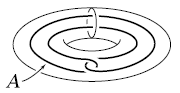
\includegraphics[scale=1]{hw3_16} \par
                $A$ is homotopic to a loop that crosses itself so it must be nullhomotopic, and thus the induced homomorphism $i_* : \pi_1(A) \to \pi_1(S^1 \times D)$ is trivial. $\pi_1(S^1 \times D)$ is not isomorphic to the trivial group, so this map is not injective.
            \item
                \boldmath\textbf{$X = D^2 \lor D^2$ with $A$ its boundary $S^1 \lor S^1$.
                }\unboldmath \par
                From the van Kampen theorem, $\pi_1(D^2 \lor D^2) \iso \{e\} * \{e\} \iso \{e\}$ while $\pi_1(S^1 \lor S^1) \iso \mathbb{Z} * \mathbb{Z}$, so the homomorphism induced by inclusion is not injective.
            \item
                \boldmath\textbf{$X$ a disk with two points on its boundary identified and $A$ its boundary $S^1 \lor S^1$.
                }\unboldmath \par
                $X$ is homotopy equivalent to $S^1$ (since there is a deformation retraction from the disk onto any arc, including the arc between the two identified points, which becomes a circle under the quotient space), which means $\pi_1(X) \iso \mathbb{Z}$, and no injection exists from $\mathbb{Z} * \mathbb{Z}$ to $\mathbb{Z}$.
            \item
                \boldmath\textbf{$X$ the M\"obius band and $A$ its boundary circle.
                }\unboldmath \par
                $\pi(X) = \mathbb{Z}$ since $X$ deformation retracts onto the M\"obius band's core circle. While $\pi(A) = \mathbb{Z}$ also, the homomorphism induced by inclusion is multiplication by 2, since a loop that travels around the boundary circle deformation retracts onto a loop that travels around the core circle twice. Then we know that the homomorphism is not injective, since no integers map onto the odd integers.
        \end{enumerate}

    \item[17.]
        \boldmath\textbf{Construct infinitely many nonhomotopic retractions $S^1 \lor S^1 \to S^1$.
        }\unboldmath \par
        Let $A, B$ denote the respective summands of $S^1 \lor S^1$, where $A$, $B$ are unit circles centered at the origin. Then we can construct retractions $r_n : A \lor B \to A$ defined by the identity map on summand $A$ and the map $(r, \theta) \mapsto (r, n\theta)$ on summand $B$. From Theorem 1.7, we know that $r_m \simeq r_n$ iff $m = n$. Thus, taking $n \in \mathbb{N}$ gives infinitely many nonhomotopic retractions.
\end{enumerate}

\subsection*{Section 1.2}
\begin{enumerate}
    \item[7.]
        \boldmath\textbf{Let $X$ be the quotient space of $S^2$ obtained by identifying the north and south poles to a single point. Put a cell complex structure on $X$ and use this to compute $\pi_1(X)$.
        }\unboldmath \par
        $X$ is composed of one $0$-cell, one $1$-cell whose endpoints (the north and south poles) are both located at the $0$-cell, and one $2$-cell whose boundary is given by the path traversing the $1$-cell and back. %Let $A, B \in X$ be sets that contain the 1-cell and the 2-cell respectively as proper subsets, such that $A \cup B = X$ and $A \cap B$ is homotopic to a $0$-cell. Then $\pi_1(A) \iso \pi_1(S^1) \iso \mathbb{Z}$ and $\pi_1(B) \iso \pi_1(S^2) \iso \{e\}$.
        The kernel of the surjection $\pi_1(X) \to \pi_1(S^2)$ induced by the inclusion map is $\pi_1(S^1) \iso \mathbb{Z}$. Thus, by part (a) of Proposition 1.26, we have that $\pi_1(S^2) \iso \pi_1(X) / \mathbb{Z} \Rightarrow \pi_1(X) \iso \mathbb{Z}$.

    %http://www.math.northwestern.edu/~pgoerss/math440/probset2/probset2.pdf
    \item[8.]
        \boldmath\textbf{Compute the fundamental group of the space obtained from two tori $S^1 \times S^1$ by identifying a circle $S^1 \times \{x_0\}$ in one torus with the corresponding circle $S^1 \times \{x_0\}$ in the other torus.
        }\unboldmath \par
        Let $A$ and $B$ denote the two tori, with $A \cap B$ containing the basepoint. Define $U$ as the union of $A$ with a small neighborhood of $A \cap B$ in $B$ that deformation retracts onto $A \cap B$, so that $U$ deformation retracts onto $A$. Similarly, define $V$ so that it deformation retracts onto $B$, giving us $\pi_1(U) \iso \pi_1(V) \iso \mathbb{Z} \times \mathbb{Z}$. Further, $U \cap V$ deformation retracts onto the circle $A \cap B$, which means $\pi_1(U \cap V) \iso \mathbb{Z}$. \par
        Under the inclusion $A \cap B \hookrightarrow A$, a generator of $\pi_1(A \cap B)$ corresponds to a loop that travels around one $S^1$ factor of $A$, and the same is true when the roles of $A$ and $B$ are reversed. Thus, $\pi_1(A)$ is an abelian free group on two generators $a$ and $b$, one for each $S^1$ factor of the torus, and similarly $\pi_1(B)$ is an abelian free group on two generators $c$ and $d$. \par
        Because the maps induced by the two inclusions have the same descriptions, we have by the van Kampen theorem that
        \begin{align*}
            \pi_1(X) &\iso \pi_1(U) *_{\pi_1(U \cap V)} \pi_1(V) \\
            &\iso \langle a, b, c, d \mid ab = ba, cd = dc, a = c \rangle \\
            &\iso \langle a, b, d \mid ab = ba, ad = da \rangle.
        \end{align*}

    \item[11.]
        \boldmath\textbf{The \emph{mapping torus} $T_f$ of a map $f : X \to X$ is the quotient of $X \times I$ obtained by identifying each point $(x, 0)$ with $(f(x), 1)$. In the case $X = S^1 \lor S^1$ with $f$ basepoint-preserving, compute a presentation for $\pi_1(T_f)$ in terms of the induced map $f_* : \pi_1(X) \to \pi_1(X)$. Do the same when $X = S^1 \times S^1$.
        }\unboldmath \par
        %Regard $T_f$ as built from $X \lor S^1$ by attaching cells.
        The $I$ factor under this identification becomes a loop $\gamma$ homeomorphic to $S^1$ attached to $S^1 \lor S^1$ at the basepoint, which is preserved under $f$, giving us $S^1 \lor S^1 \lor S^1$. Let $a$ and $b$ be generators corresponding to each of the $S^1$ summands making up $X$. What remains are two $2$-cells to be attached, which are described as follows -- the boundary of the first travels along $a$, $\gamma$, $f_*^{-1}(a)$, and finally $\gamma^{-1}$ before returning to its starting point, while the boundary of the second travels along $b$, $\gamma$, $f_*^{-1}(b)$, and $\gamma^{-1}$. The presentation is thus $\pi_1(T_f) \iso \langle a, b, \gamma \mid a \gamma f_*^{-1}(a) \gamma^{-1}, b \gamma f_*^{-1}(b) \gamma^{-1} \rangle$. \par
        \sloppy
        In the latter case, $X$ is generated by $a$ and $b$ subject to a new constraint $aba^{-1}b^{-1} = 1$, which also implies $f_*(a) f_*(b) f_*^{-1}(a) f_*^{-1}(b) = 1$. The loop $\gamma$ is attached in the same way as before, and the $2$-cells as well. A $3$-cell is now required, but it does not change $\pi_1(T_f)$. We conclude that the presentation is $\pi_1(T_f) \iso \langle a, b, \gamma \mid a \gamma f_*^{-1}(a) \gamma^{-1}, b \gamma f_*^{-1}(b) \gamma^{-1}, aba^{-1}b^{-1} \rangle$.

    \item[21.]
        \boldmath\textbf{Show that the join $X * Y$ of two nonempty spaces $X$ and $Y$ is simply-connected if $X$ is path-connected.
        }\unboldmath \par
        Let $\{Y_i\}$ be the decomposition of $Y$ into path-connected components. We will first show that proving the simple-connectedness of each $X * Y_i$ suffices to show that $X * Y$ is simply-connected through an application of the van Kampen theorem. First, let $Z$ be the restriction of $X * Y$ to $X \times Y \times [0, 1/2)$. $Z$ is path-connected because it deformation retracts onto $X$. Now let $A_i = Z \cup (X * Y_i)$; the intersection of any of these $A_i$ is $Z$. It remains to show that for any path $f$ in $X * Y$, $f^{-1}(A_i)$ is open in $I$. Since $Z$ is open in $X * Y$, $f^{-1}(Z)$ is open. Now take any point $f(s)$ in the restriction of $X * Y_i$ to $X \times Y \times (0, 1]$, which is open. Since $f$ is continuous, there exists some $\delta > 0$ such that $f((s - \delta, s + \delta)) \subset X \times Y \times (0, 1]$, and furthermore $f$ is a path so $f((s - \delta, s + \delta)) \subset A_i$. \par
        Now we must show that $X * Y_i$ is simply-connected, adopting the notation $Y$ in place of $Y_i$ hereafter. We can write $X * Y = Z_1 \cup Z_2$ where $Z_1$ is $X * Y$ restricted to $X \times Y \times [0, 2/3]$ and $Z_2$ is the same restricted to $X \times Y \times (1/3, 1]$. We know that $Z_1$ and $Z_2$ deformation retract onto $X$ and $Y$ respectively, and $Z_1 \cap Z_2$ deformation retracts onto $X \times Y$. Given the inclusion maps $i_1 : X \times Y \to Z_1$ and $i_2 : X \times Y \to Z_2$, the van Kampen theorem states that $\pi_1(X * Y)$ is the quotient of $\pi_1(X) * \pi_1(Y)$ by the subgroup generated by the $i_{1*}(x, y) i_{2*}(x, y)^{-1}$, which include $xy^{-1}$ for all $x \in X, y \in Y$. We can deduce that $\pi_1(X * Y) = \{e\}$, and in conclusion $X * Y$ is simply-connected.

    %http://math.stackexchange.com/questions/928930/obtaining-wirtinger-presentation-using-van-kampen-theorem
    %http://homepages.math.uic.edu/~kauffman/Stillwell.pdf
    %http://math.stackexchange.com/questions/1563549/what-is-the-abelianization-of-pi-1-mathbbr3-setminus-k-where-k-is-a-k/1568603#1568603
    \item[22.]
        \boldmath\textbf{Consider the \emph{Wirtinger presentation} of the fundamental group of the complement of a smooth or piecewise linear knot $K$ in $\mathbb{R}^3$.
        }\unboldmath \par
        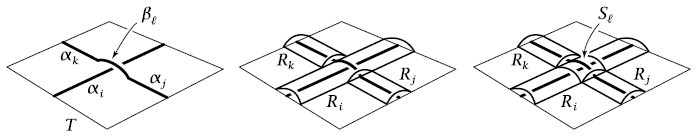
\includegraphics[scale=0.75]{hw3_22} \par
        \begin{enumerate}[label=(\alph*)]
            \item
                \boldmath\textbf{Show that $\pi_1(\mathbb{R}^3 - K)$ has a presentation with one generator $x_i$ for each strip $R_i$ and one relation of the form $x_i x_j x_i^{-1} = x_k$ for each square $S_l$, where the indices are as in the figures above.
                }\unboldmath \par
                For each strip $R_i$, there is a corresponding generator $a_i$ that passes around the arc $\alpha_i$, which can be seen from applying the van Kampen theorem. We can choose to orient the generators using the right-hand rule where the positions of $R_i$ and $R_j$ relative to $S_l$ determine the positive directions. By tracing out a loop that passes along the arcs surrounding $S_l$, we can deduce the relation $x_i x_j x_i^{-1} x_k^{-1} = 1$, or $x_i x_j x_i^{-1} = x_k$.

            \item
                \boldmath\textbf{Use this presentation to show that the abelianization of $\pi(\mathbb{R}^3 - K)$ is $\mathbb{Z}$.
                }\unboldmath \par
                Since abelianization is the same as introducing the relator $x_i x_j x_i^{-1} = x_j$, which when combined with the previous relator implies that $x_j = x_k$ for all $x_k$, we can deduce that the abelianization has a unique generator, so it is infinite cyclic and hence isomorphic to $\mathbb{Z}$.
        \end{enumerate}
\end{enumerate}
\end{document}
